\usetikzlibrary{arrows.meta,positioning,calc,shapes.geometric}
\definecolor{delta_color}{RGB}{242,243,193}
\definecolor{swa_color}{RGB}{252,224,225}
\definecolor{glu_color}{RGB}{194,232,247}
\definecolor{silu_color}{RGB}{203,231,207}
\definecolor{linear_color}{RGB}{220,223,240}
\definecolor{conv_color}{RGB}{252,224,225}
\definecolor{gray_bbox_color}{RGB}{243,243,244}
\begin{figure*}[!t]
\centering
\vspace{15pt}
\tikzset{
  model/.style={
    draw=black, very thick, fill=gray_bbox_color,
    minimum width=96pt, rounded corners=8pt
  },
  gdelta/.style={
    draw=black, very thick, fill=gray_bbox_color,
    minimum width=120pt, minimum height=190pt, rounded corners=10pt
  },
  swa/.style={
    draw=black, very thick, fill=swa_color!80,
    minimum width=78pt, minimum height=0.7cm, rounded corners=3pt
  },
  glu/.style={
    draw=black, very thick, fill=glu_color!80,
    minimum width=78pt, minimum height=0.7cm, rounded corners=3pt
  },
  conv/.style={
    draw=black, very thick, minimum width=50pt, minimum height=20pt,
    fill=conv_color!80, rounded corners=3pt
  },
  linear/.style={
    draw=black, very thick, trapezium,
    trapezium left angle=110, trapezium right angle=110,
    minimum width=50pt, minimum height=15pt, fill=linear_color!80
  },
  branch_node/.style={
    draw=black, very thick, minimum width=40pt, minimum height=15pt,
    fill=linear_color!80, rounded corners=3pt
  },
  silu/.style={
    draw=black, very thick, fill=silu_color,
    minimum width=35pt, minimum height=12pt, rounded corners=3pt
  },
  layerlink/.style={-latex, line width=0.6pt},
  modulelink/.style={-latex, very thick, densely dashed},
  normlink/.style={very thick},
  otimes/.style={
    draw=black, very thick, circle, minimum size=11pt,
    inner sep=0pt, outer sep=0pt,
    path picture={
      \draw (path picture bounding box.center) -- ++(0.25cm,0.25cm)
            (path picture bounding box.center) -- ++(-0.25cm,-0.25cm)
            (path picture bounding box.center) -- ++(-0.25cm,0.25cm)
            (path picture bounding box.center) -- ++(0.25cm,-0.25cm);
    }
  },
  gradlink/.style={very thick, grad_color, -{Latex[length=3mm]}},
  stopgrad/.style={
    fill=gray_bbox_color,
    draw=grad_color, very thick, circle, minimum size=10pt, inner sep=0pt,
    path picture={
      \draw[grad_color, very thick]
        (path picture bounding box.south west) -- (path picture bounding box.north east)
        (path picture bounding box.north west) -- (path picture bounding box.south east);
    }
  }
}

\definecolor{grad_color}{RGB}{220,70,70}


\scalebox{0.85}{
\centering
\resizebox{0.7\textwidth}{!}{

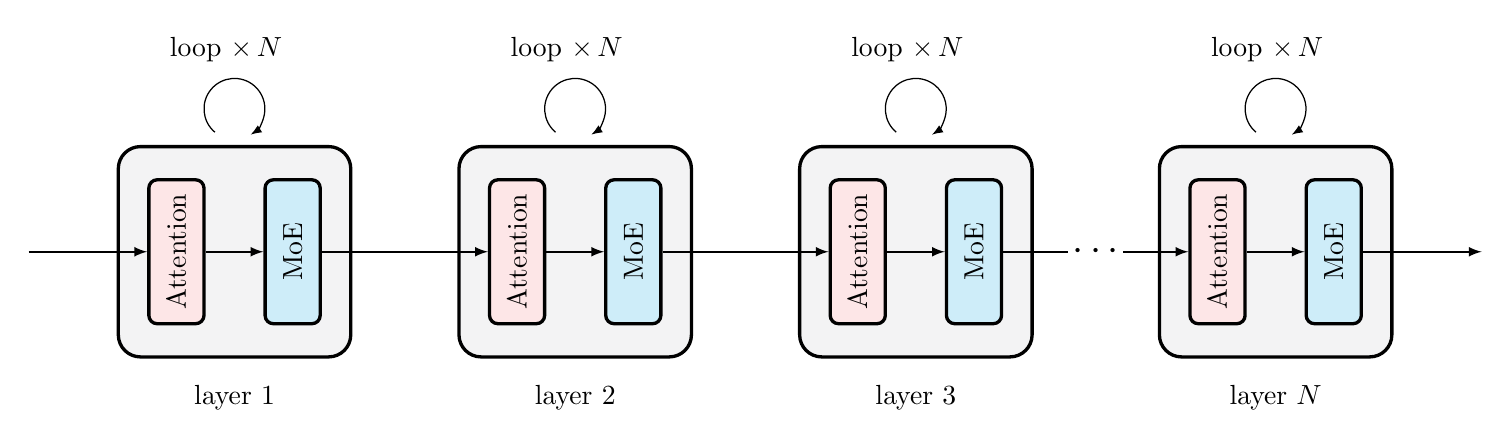
\begin{tikzpicture}

\node[model, minimum width=84pt, minimum height=76pt] (model1) at (0,0) {};
\node[below=6pt, align=center] at (model1.south) {layer 1};
\node[swa, minimum width=0.7cm, minimum height=52pt] (attn1) at ($(model1.center) + (-21pt, 0)$) {\rotatebox{90}{Attention}};
\node[glu, minimum width=0.7cm, minimum height=52pt] (moe1) at ($(model1.center) + (21pt, 0)$) {\rotatebox{90}{MoE}};

\node[model, minimum width=84pt, minimum height=76pt] (model2) at (123.1pt,0) {};
\node[below=6pt, align=center] at (model2.south) {layer 2};
\node[swa, minimum width=0.7cm, minimum height=52pt] (attn2) at ($(model2.center) + (-21pt, 0)$) {\rotatebox{90}{Attention}};
\node[glu, minimum width=0.7cm, minimum height=52pt] (moe2) at ($(model2.center) + (21pt, 0)$) {\rotatebox{90}{MoE}};

\node[model, minimum width=84pt, minimum height=76pt] (model3) at (246.2pt,0) {};
\node[below=6pt, align=center] at (model3.south) {layer 3};
\node[swa, minimum width=0.7cm, minimum height=52pt] (attn3) at ($(model3.center) + (-21pt, 0)$) {\rotatebox{90}{Attention}};
\node[glu, minimum width=0.7cm, minimum height=52pt] (moe3) at ($(model3.center) + (21pt, 0)$) {\rotatebox{90}{MoE}};

\node[model, minimum width=84pt, minimum height=76pt] (model4) at (376.2pt,0) {};
\node[below=6pt, align=center] at (model4.south) {layer $N$};
\node[swa, minimum width=0.7cm, minimum height=52pt] (attn4) at ($(model4.center) + (-21pt, 0)$) {\rotatebox{90}{Attention}};
\node[glu, minimum width=0.7cm, minimum height=52pt] (moe4) at ($(model4.center) + (21pt, 0)$) {\rotatebox{90}{MoE}};

\draw[-{Latex[length=1.4mm]}, line width=0.45pt] ($(model1.north) + (-7.1pt, 4.6pt)$) arc[start angle=230, end angle=-58, radius=11pt] node[pos=0.43, above=3pt] {loop $\times\, N$};
\draw[-{Latex[length=1.4mm]}, line width=0.45pt] ($(model2.north) + (-7.1pt, 4.6pt)$) arc[start angle=230, end angle=-58, radius=11pt] node[pos=0.43, above=3pt] {loop $\times\, N$};
\draw[-{Latex[length=1.4mm]}, line width=0.45pt] ($(model3.north) + (-7.1pt, 4.6pt)$) arc[start angle=230, end angle=-58, radius=11pt] node[pos=0.43, above=3pt] {loop $\times\, N$};
\draw[-{Latex[length=1.4mm]}, line width=0.45pt] ($(model4.north) + (-7.1pt, 4.6pt)$) arc[start angle=230, end angle=-58, radius=11pt] node[pos=0.43, above=3pt] {loop $\times\, N$};

\coordinate (left_input_start) at ($(model1.west) + (-31.85pt, 0)$);
\coordinate (right_output_end) at ($(model4.east) + (31.85pt, 0)$);
\node[anchor=east, align=center, font=\bfseries\large, overlay] at ($(left_input_start) + (-14pt, 0)$) {Layer-loop};
\draw[layerlink] (left_input_start) -- (attn1.west);
\draw[layerlink] (attn1.east) -- (moe1.west);
\draw[layerlink] (moe1.east) -- (attn2.west);
\draw[layerlink] (attn2.east) -- (moe2.west);
\draw[layerlink] (moe2.east) -- (attn3.west);
\draw[layerlink] (attn3.east) -- (moe3.west);
\draw[layerlink] (moe3.east) -- node[midway, fill=white, inner sep=1.5pt, font=\Large] {$\cdots$} (attn4.west);
\draw[layerlink] (attn4.east) -- (moe4.west);
\draw[layerlink] (moe4.east) -- (right_output_end);

\end{tikzpicture}
}

}
\par\vspace{5mm}
\noindent\makebox[\textwidth][c]{%
\raisebox{6mm}{%
\tikz\draw[gray!70, densely dashed, line width=0.6pt] (0,0) -- (\textwidth,0);
}%
}
\raisebox{5mm}{\scalebox{0.85}{
\centering
\resizebox{0.7\textwidth}{!}{

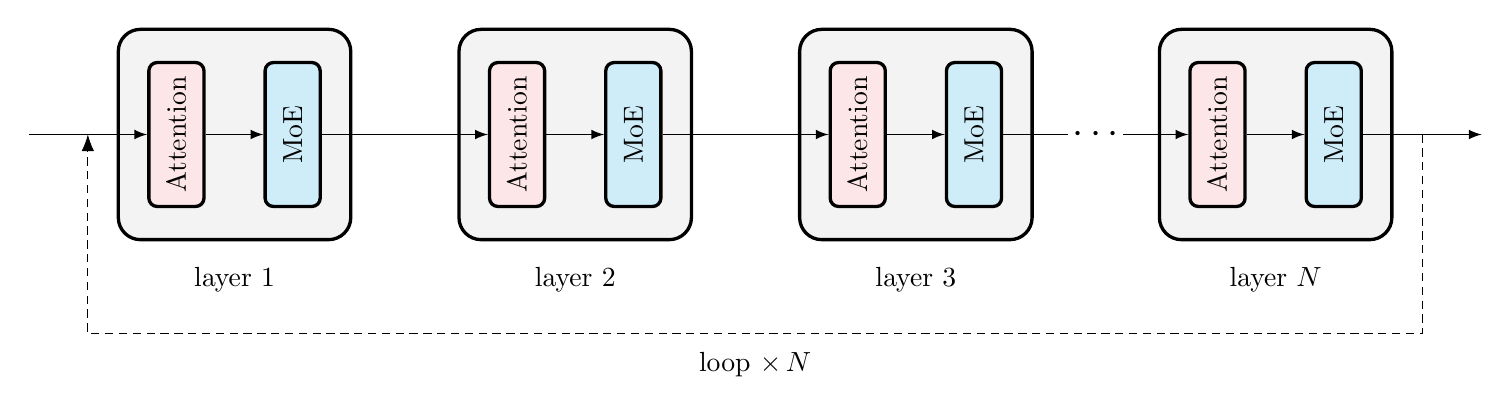
\begin{tikzpicture}

\node[model, minimum width=84pt, minimum height=76pt] (model1) at (0,0) {};
\node[below=6pt, align=center] at (model1.south) {layer 1};
\node[swa, minimum width=0.7cm, minimum height=52pt] (attn1) at ($(model1.center) + (-21pt, 0)$) {\rotatebox{90}{Attention}};
\node[glu, minimum width=0.7cm, minimum height=52pt] (moe1) at ($(model1.center) + (21pt, 0)$) {\rotatebox{90}{MoE}};

\node[model, minimum width=84pt, minimum height=76pt] (model2) at (123.1pt,0) {};
\node[below=6pt, align=center] at (model2.south) {layer 2};
\node[swa, minimum width=0.7cm, minimum height=52pt] (attn2) at ($(model2.center) + (-21pt, 0)$) {\rotatebox{90}{Attention}};
\node[glu, minimum width=0.7cm, minimum height=52pt] (moe2) at ($(model2.center) + (21pt, 0)$) {\rotatebox{90}{MoE}};

\node[model, minimum width=84pt, minimum height=76pt] (model3) at (246.2pt,0) {};
\node[below=6pt, align=center] at (model3.south) {layer 3};
\node[swa, minimum width=0.7cm, minimum height=52pt] (attn3) at ($(model3.center) + (-21pt, 0)$) {\rotatebox{90}{Attention}};
\node[glu, minimum width=0.7cm, minimum height=52pt] (moe3) at ($(model3.center) + (21pt, 0)$) {\rotatebox{90}{MoE}};

\node[model, minimum width=84pt, minimum height=76pt] (model4) at (376.2pt,0) {};
\node[below=6pt, align=center] at (model4.south) {layer $N$};
\node[swa, minimum width=0.7cm, minimum height=52pt] (attn4) at ($(model4.center) + (-21pt, 0)$) {\rotatebox{90}{Attention}};
\node[glu, minimum width=0.7cm, minimum height=52pt] (moe4) at ($(model4.center) + (21pt, 0)$) {\rotatebox{90}{MoE}};


\coordinate (left_input_start) at ($(model1.west) + (-31.85pt, 0)$);
\coordinate (right_output_end) at ($(model4.east) + (31.85pt, 0)$);
\coordinate (skip_input) at ($(left_input_start)!0.5!(attn1.west)$);
\coordinate (skip_output) at ($(moe4.east)!0.5!(right_output_end)$);
\node[anchor=east, align=center, font=\bfseries\large, overlay] at ($(left_input_start) + (-14pt, 0)$) {Model-loop};
\draw[layerlink] (left_input_start) -- (attn1.west);
\draw[layerlink] (attn1.east) -- (moe1.west);
\draw[layerlink] (moe1.east) -- (attn2.west);
\draw[layerlink] (attn2.east) -- (moe2.west);
\draw[layerlink] (moe2.east) -- (attn3.west);
\draw[layerlink] (attn3.east) -- (moe3.west);
\draw[layerlink] (moe3.east) -- node[midway, fill=white, inner sep=1.5pt, font=\Large] {$\cdots$} (attn4.west);
\draw[layerlink] (attn4.east) -- (moe4.west);
\draw[layerlink] (moe4.east) -- (right_output_end);
\coordinate (model_loop_bottom_left) at ($(skip_input) + (0,-72pt)$);
\coordinate (model_loop_bottom_right) at ($(skip_output) + (0,-72pt)$);
\draw[-{Latex[length=2.1mm]}, black, densely dashed, line width=0.32pt] (skip_output) -- (model_loop_bottom_right) -- (model_loop_bottom_left) -- (skip_input);
\node[below=3pt] at ($(model_loop_bottom_left)!0.5!(model_loop_bottom_right)$) {loop $\times\, N$};

\end{tikzpicture}
}
}}
\vspace{3mm}
\caption{Illustration of the contrast between \textbf{layer-loop} and \textbf{model-loop}. The top panel shows layer-loop, the loop schedule adopted by Loopie, in which each Attention/MoE layer is applied recurrently before passing its output to the next layer. We demonstrate that this schedule achieves better performance on MoE backbones while also training more efficiently. The bottom panel shows the traditional whole-model recurrence pattern, which we call model-loop, where the entire layer stack is traversed and then repeated. This pattern is used by prior looped models such as Ouro and Huginn \citep{zhu2025scalinglatent,geiping2025scalinglatent}.}
\label{fig:layer-vs-model-loop}
\end{figure*}
